\documentclass{beamer}

% Theme choice
\usetheme{Madrid}
\usecolortheme{default}

% Packages
\usepackage{graphicx}
\usepackage{amsmath, amssymb}
\usepackage{booktabs}
\usepackage{tikz}
\usetikzlibrary{positioning, arrows.meta, fit}

% Title info
\title{Bayesian Latent Variable Model of Economic Activity in Cuba}
\author{Christopher M. Perez}
\date{May 6, 2025}

\begin{document}

% TITLE SLIDE
\begin{frame}
  \titlepage
\end{frame}

% NEWS SLIDES with stacked bordered images
\begin{frame}{What's Really Happening in Cuba?}
  \centering
  \fbox{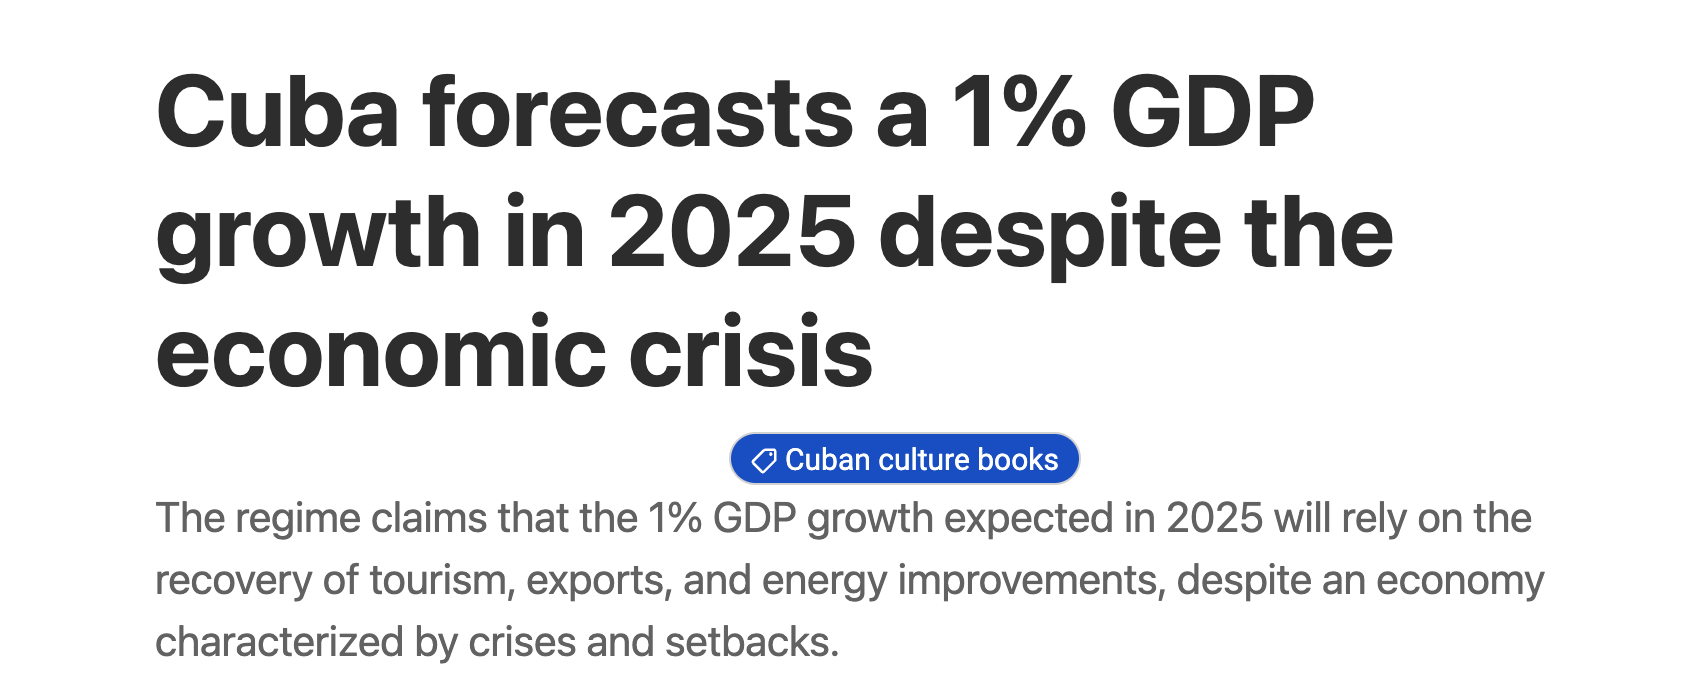
\includegraphics[width=0.8\textwidth]{/Users/chrisperez/Desktop/stat288-finalproject/images/news_1.png}} \\[1em]
  \fbox{
\includegraphics[width=0.8\textwidth]{/Users/chrisperez/Desktop/stat288-finalproject/images/news_3.png}}
\end{frame}

\begin{frame}{What's Really Happening in Cuba?}
  \centering
  \fbox{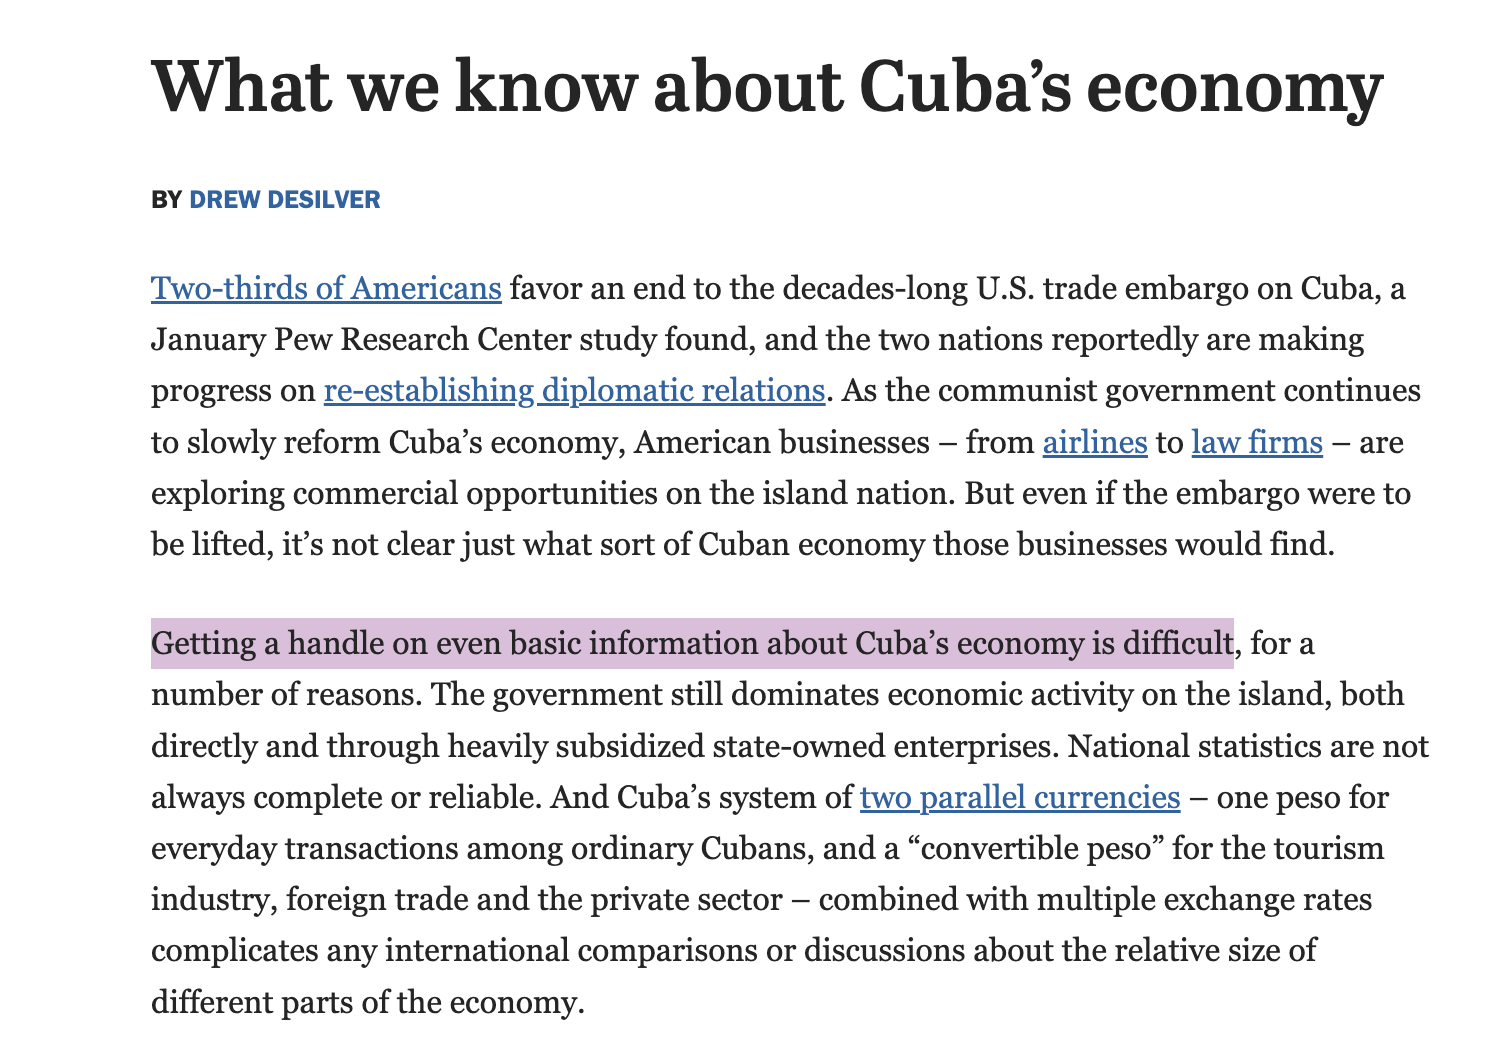
\includegraphics[width=0.8\textwidth]{/Users/chrisperez/Desktop/stat288-finalproject/images/news_4.png}}
\end{frame}


% MOTIVATION & CONTEXT
\begin{frame}{Motivation}
\begin{itemize}
  \item Reliable economic data for Cuba is scarce and disputed.
  \item Traditional indicators (e.g., GDP) are not consistently reported.
  \item Can we infer economic activity using satellite imagery and open data?
\end{itemize}
\end{frame}

\begin{frame}{Research Question}
\begin{block}{Goal}
Estimate a latent index of economic activity across Cuba using spatial proxies.
\end{block}
\pause
\begin{itemize}
  \item Combine nightlights, NDVI, and road density data
  \item Use a Bayesian model to infer unobserved economic activity
\end{itemize}
\end{frame}

% DATA SOURCES
\begin{frame}{Data Sources}
\begin{itemize}
    \item \textbf{Nighttime Lights (VIIRS)}: Proxy for infrastructure \& development.
    \item \textbf{NDVI}: Measures vegetation ``greenness."
  \item \textbf{Road Density}: Infrastructure connectivity.
\end{itemize}
\pause
All proxies standardized and aligned to 500m grid. Water masked out.
\end{frame}

% MODEL OVERVIEW
\begin{frame}{Bayesian Hierarchical Model}
\begin{itemize}
  \item Latent economic activity $z_i$ per grid cell
  \item Observed proxies $x_{i,k} \sim \mathcal{N}(\beta_k z_i, \sigma_k^2)$
  \item Fixed $\beta_{\text{lights}} = 1$ for identifiability
  \item Spatial prior on $z$
\end{itemize}
\end{frame}

\begin{frame}{Graphical Model}
\centering

\includegraphics[width=0.8\textwidth]{/Users/chrisperez/Desktop/stat288-finalproject/images/plate.png}
\end{frame}

% POSTERIOR RESULTS
\begin{frame}{Posterior Results: Cuba (15km Grid)}
\begin{itemize}
  \item Posterior mean of $z_i$ shown below:
\end{itemize}
\centering
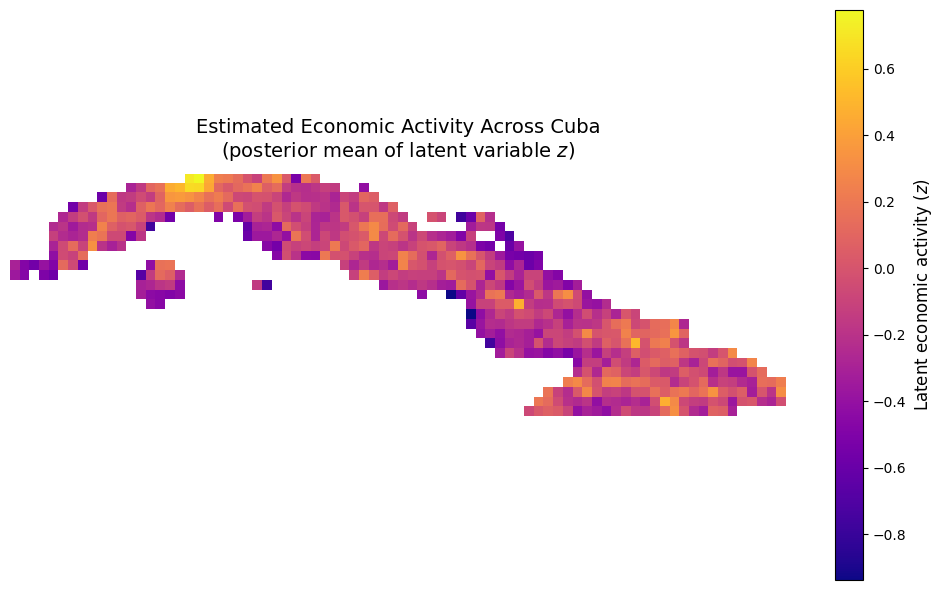
\includegraphics[width=0.6\textwidth]{/Users/chrisperez/Desktop/stat288-finalproject/images/fig1.png}
\end{frame}

\begin{frame}{Uncertainty Estimates}
\begin{itemize}
  \item Posterior standard deviation is low ($\approx$ 0.04--0.06)
  \item Higher uncertainty in urban areas like Havana
\end{itemize}
\centering
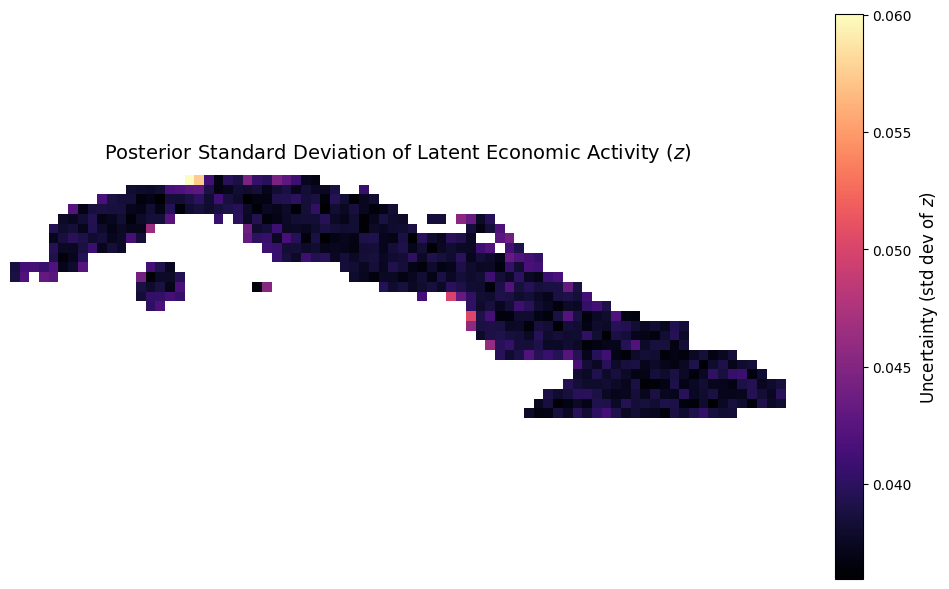
\includegraphics[width=0.6\textwidth]{/Users/chrisperez/Desktop/stat288-finalproject/images/fig2.png}
\end{frame}

% COEFFICIENTS & DIAGNOSTICS
\begin{frame}{Model Coefficients}
\centering
\begin{itemize}
  \item $\beta_{\text{NDVI}} \approx 0.14$ (weakly positive)
  \item $\beta_{\text{roads}} \approx 2.29$ (strong positive)
  \item $\sigma$ values show road is low-noise; NDVI is high-noise
\end{itemize}
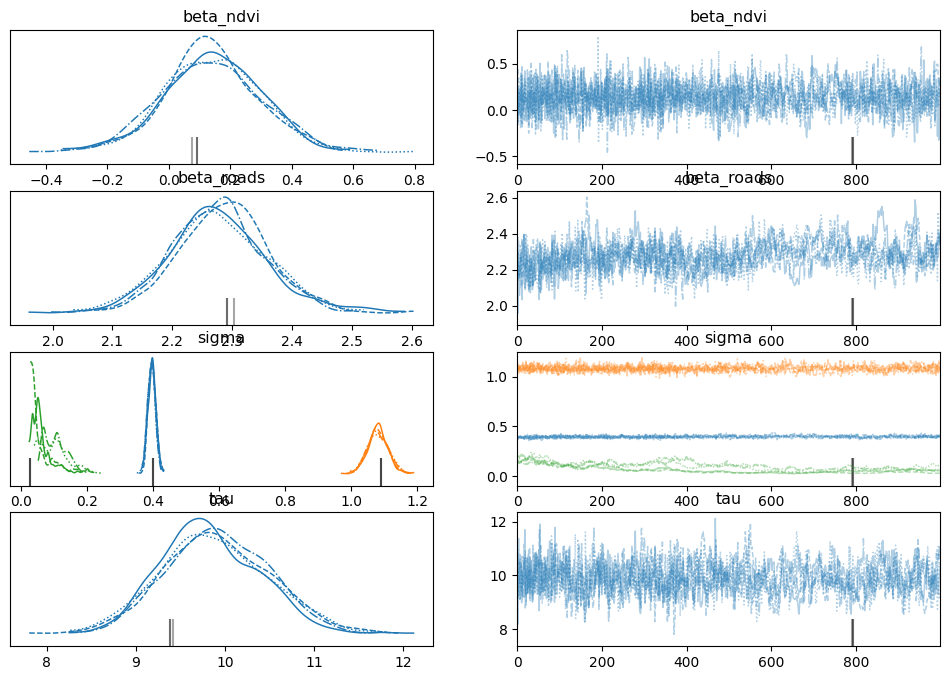
\includegraphics[width=0.7\textwidth]{/Users/chrisperez/Desktop/stat288-finalproject/images/fig_3_post_diagnostics.png}
\end{frame}

% MULTI-RESOLUTION
\begin{frame}{Multi-Resolution Analysis}
\begin{itemize}
  \item Refit model at 5 km, 10 km, 20 km grids
  \item Observe stable coefficients but varied uncertainty
  \item $\beta_{\text{NDVI}}$ flips sign across resolutions
\end{itemize}
\end{frame}

\begin{frame}{Resolution Comparison: Maps}
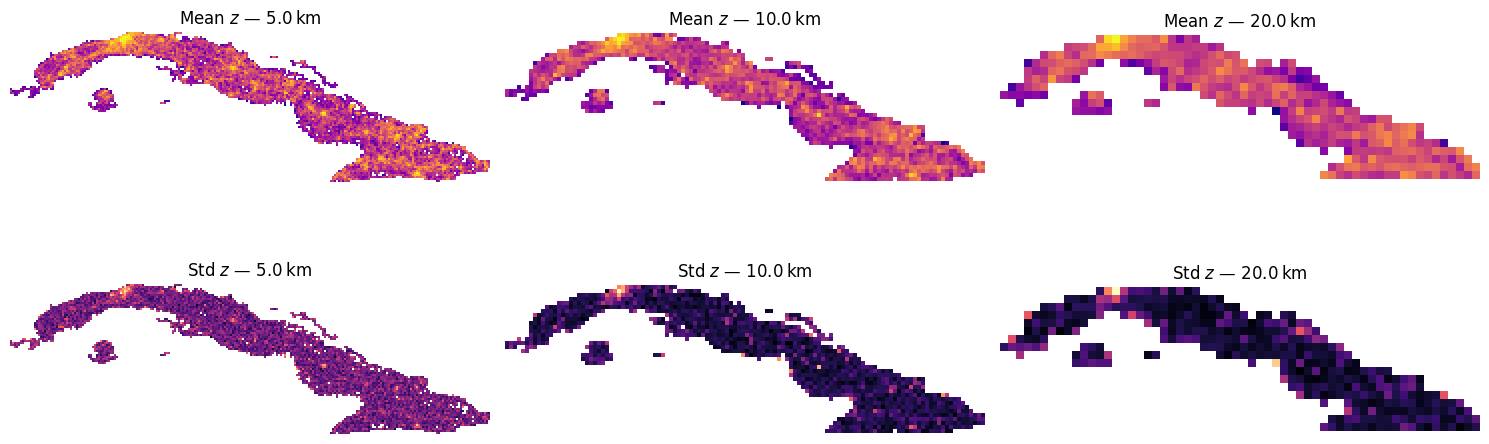
\includegraphics[width=\textwidth]{/Users/chrisperez/Desktop/stat288-finalproject/images/multires_cuba.png}
\end{frame}

\begin{frame}{Zoom-In: Greater Havana and Camagüey}
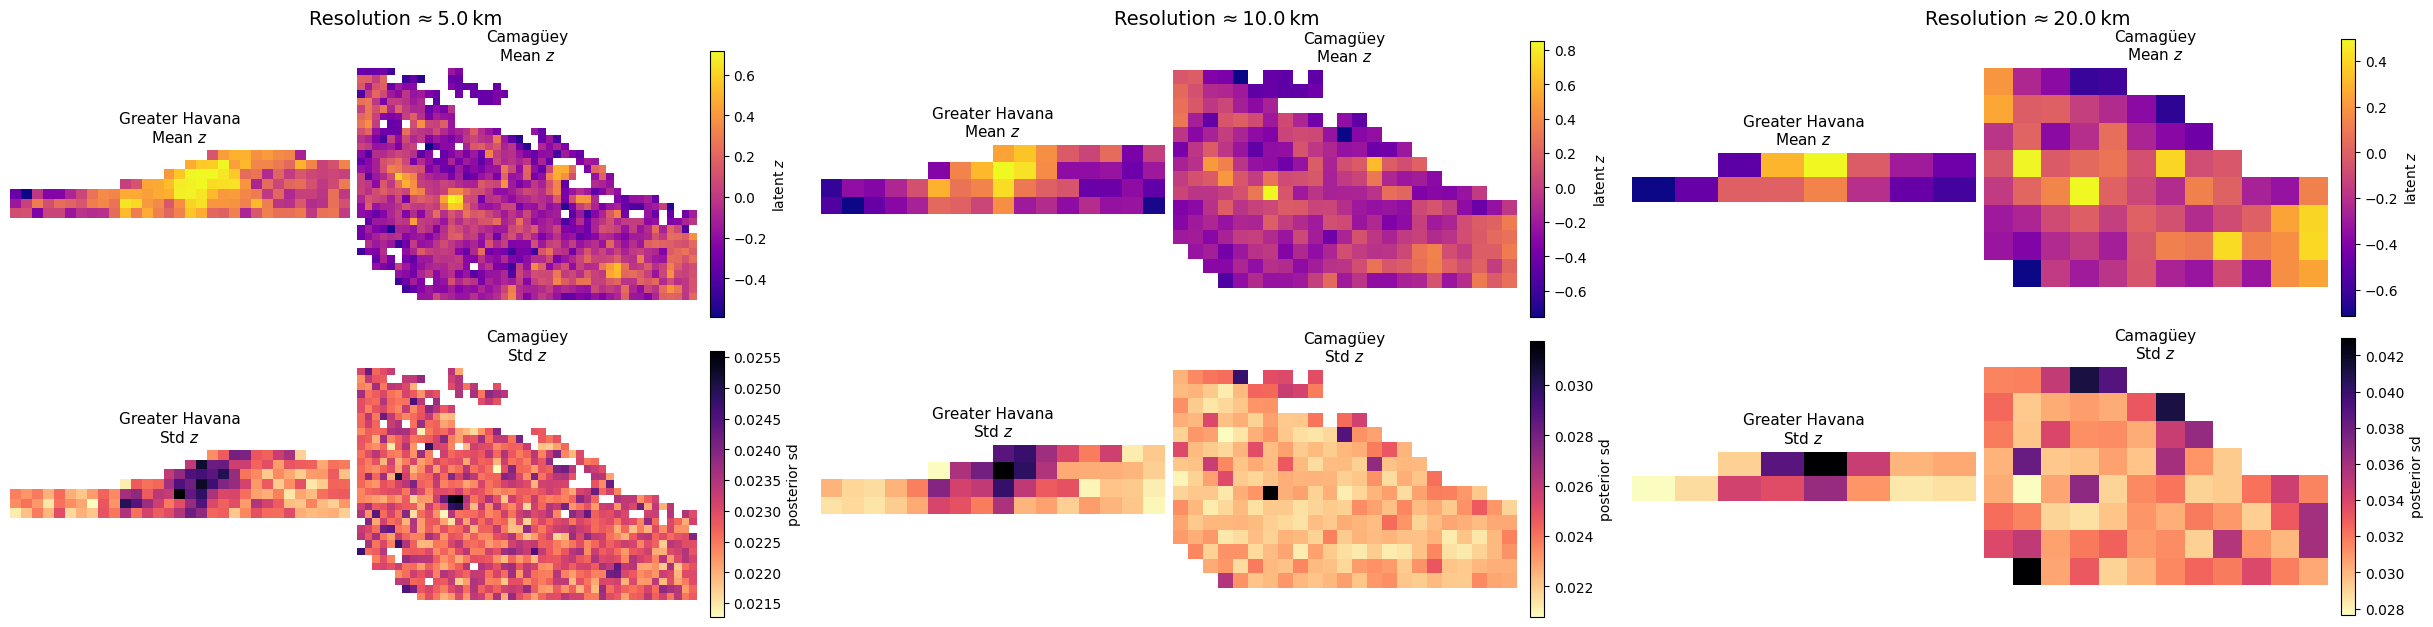
\includegraphics[width=\textwidth]{/Users/chrisperez/Desktop/stat288-finalproject/images/combined_maps.png}
\end{frame}


% CONCLUSION
\begin{frame}{Conclusion and Future Work}
\begin{itemize}
  \item Nightlights + roads = best proxies for economic activity in Cuba
  \item Bayesian model provides uncertainty-aware estimates
  \item Limitations: No ground-truth calibration, constant coefficients
  \item Immediate Next Step: Validate model on Dominican Republic
  \item Future: Add time dimension
\end{itemize}
\end{frame}

\end{document}
